\SourceLeaf{175}\begin{center}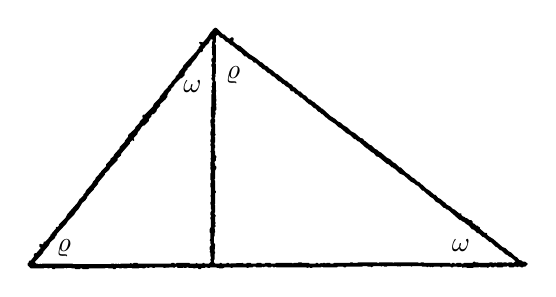
\begin{tikzpicture}[x=0.00778923cm,y=-0.00778923cm]
\fill[even odd rule] (31,407) -- (36,412) -- (57,412) -- (58,411) -- (63,411) -- (64,412) -- (66,412) -- (67,411) -- (70,411) -- (72,413) -- (75,413) -- (76,412) -- (90,412) -- (91,411) -- (93,411) -- (94,412) -- (96,411) -- (102,411) -- (103,412) -- (108,412) -- (109,413) -- (116,413) -- (117,412) -- (120,412) -- (121,413) -- (130,413) -- (131,412) -- (157,412) -- (158,411) -- (162,411) -- (163,412) -- (170,412) -- (171,413) -- (174,413) -- (176,411) -- (180,411) -- (181,412) -- (184,412) -- (185,411) -- (187,411) -- (188,412) -- (193,412) -- (194,411) -- (201,411) -- (202,412) -- (212,412) -- (213,411) -- (218,411) -- (219,412) -- (221,412) -- (225,410) -- (227,411) -- (229,411) -- (230,410) -- (234,410) -- (235,411) -- (238,411) -- (239,410) -- (252,410) -- (253,411) -- (268,410) -- (270,411) -- (273,409) -- (274,409) -- (276,411) -- (284,411) -- (285,410) -- (286,411) -- (290,411) -- (291,410) -- (293,410) -- (294,411) -- (301,411) -- (302,412) -- (308,411) -- (310,413) -- (313,413) -- (315,411) -- (320,411) -- (321,410) -- (324,410) -- (325,411) -- (328,411) -- (329,410) -- (339,410) -- (340,411) -- (343,411) -- (344,412) -- (349,412) -- (353,410) -- (362,410) -- (363,411) -- (365,411) -- (366,410) -- (388,410) -- (389,411) -- (391,411) -- (392,410) -- (398,410) -- (399,409) -- (403,409) -- (404,410) -- (413,410) -- (414,409) -- (416,410) -- (418,409) -- (422,409) -- (423,410) -- (428,410) -- (429,409) -- (431,409) -- (432,410) -- (434,410) -- (435,409) -- (437,410) -- (486,410) -- (487,411) -- (491,410) -- (492,411) -- (495,411) -- (496,410) -- (510,410) -- (511,409) -- (513,410) -- (536,410) -- (537,409) -- (546,409) -- (547,410) -- (550,410) -- (551,409) -- (577,409) -- (578,408) -- (585,408) -- (586,409) -- (591,409) -- (592,410) -- (596,408) -- (607,408) -- (608,409) -- (610,408) -- (612,408) -- (613,409) -- (617,409) -- (618,408) -- (634,408) -- (635,409) -- (637,408) -- (639,409) -- (641,408) -- (656,408) -- (657,409) -- (659,408) -- (674,408) -- (675,409) -- (682,409) -- (683,410) -- (685,409) -- (687,409) -- (688,410) -- (690,409) -- (692,410) -- (694,409) -- (704,409) -- (705,410) -- (707,410) -- (708,409) -- (721,409) -- (722,410) -- (725,410) -- (726,409) -- (732,409) -- (733,410) -- (739,409) -- (741,411) -- (743,410) -- (747,410) -- (748,411) -- (758,411) -- (759,410) -- (767,410) -- (769,409) -- (770,410) -- (780,410) -- (782,411) -- (785,409) -- (787,409) -- (788,410) -- (792,410) -- (793,409) -- (796,409) -- (797,410) -- (806,410) -- (807,409) -- (813,409) -- (814,408) -- (815,408) -- (817,410) -- (824,410) -- (825,409) -- (829,409) -- (830,410) -- (832,409) -- (835,409) -- (836,410) -- (839,410) -- (840,409) -- (843,409) -- (847,405) -- (847,404) -- (843,401) -- (839,401) -- (837,399) -- (833,398) -- (830,394) -- (826,392) -- (820,386) -- (816,384) -- (811,379) -- (806,377) -- (791,364) -- (783,359) -- (781,357) -- (781,355) -- (780,354) -- (777,354) -- (769,347) -- (769,345) -- (768,344) -- (767,344) -- (765,342) -- (763,342) -- (760,339) -- (759,339) -- (757,337) -- (757,335) -- (755,333) -- (752,333) -- (748,330) -- (746,330) -- (744,328) -- (741,327) -- (739,325) -- (739,323) -- (738,322) -- (735,322) -- (728,316) -- (725,315) -- (721,311) -- (715,308) -- (712,304) -- (711,304) -- (704,298) -- (701,297) -- (697,292) -- (695,292) -- (687,285) -- (682,282) -- (675,275) -- (674,275) -- (670,271) -- (667,270) -- (662,265) -- (658,263) -- (654,259) -- (649,256) -- (640,247) -- (638,247) -- (632,241) -- (628,239) -- (623,234) -- (617,231) -- (608,223) -- (604,221) -- (601,218) -- (598,217) -- (592,211) -- (589,210) -- (582,204) -- (581,204) -- (578,200) -- (574,199) -- (565,191) -- (559,188) -- (553,182) -- (546,178) -- (542,174) -- (537,172) -- (533,168) -- (525,163) -- (512,151) -- (511,151) -- (504,145) -- (503,145) -- (498,140) -- (497,140) -- (492,136) -- (490,136) -- (485,130) -- (482,129) -- (476,123) -- (474,123) -- (468,117) -- (465,116) -- (462,112) -- (458,110) -- (454,106) -- (451,105) -- (439,95) -- (436,94) -- (431,89) -- (426,86) -- (422,82) -- (419,81) -- (414,76) -- (411,75) -- (404,69) -- (393,62) -- (378,49) -- (373,47) -- (366,41) -- (367,39) -- (367,36) -- (366,35) -- (363,35) -- (361,37) -- (358,36) -- (352,30) -- (350,30) -- (340,20) -- (337,19) -- (333,22) -- (333,23) -- (329,27) -- (324,35) -- (318,42) -- (316,43) -- (312,42) -- (311,43) -- (311,44) -- (313,46) -- (313,48) -- (310,51) -- (310,53) -- (307,56) -- (307,57) -- (285,81) -- (284,84) -- (278,91) -- (277,94) -- (273,98) -- (272,101) -- (266,107) -- (265,110) -- (260,115) -- (260,116) -- (253,123) -- (253,124) -- (247,131) -- (246,134) -- (237,143) -- (235,148) -- (222,161) -- (220,161) -- (218,163) -- (219,167) -- (214,172) -- (213,175) -- (207,181) -- (206,184) -- (195,194) -- (195,197) -- (190,203) -- (189,206) -- (181,214) -- (181,216) -- (172,226) -- (171,229) -- (166,233) -- (166,235) -- (159,242) -- (159,245) -- (151,253) -- (151,254) -- (147,258) -- (147,259) -- (142,264) -- (141,267) -- (138,270) -- (136,274) -- (126,285) -- (125,288) -- (122,291) -- (122,293) -- (117,298) -- (116,298) -- (112,305) -- (96,323) -- (93,329) -- (82,340) -- (82,342) -- (80,344) -- (78,344) -- (77,345) -- (77,347) -- (70,355) -- (70,356) -- (68,357) -- (68,359) -- (65,362) -- (65,363) -- (60,368) -- (58,368) -- (57,369) -- (57,371) -- (55,373) -- (53,372) -- (51,372) -- (50,373) -- (50,376) -- (52,378) -- (52,379) -- (45,387) -- (43,387) -- (41,389) -- (41,393) -- (36,399) -- (34,399) -- (33,400) -- (33,402) -- (31,404) -- cycle
(332,38) -- (333,39) -- (333,41) -- (332,42) -- (332,49) -- (331,51) -- (332,52) -- (332,63) -- (333,64) -- (333,68) -- (331,70) -- (331,74) -- (332,75) -- (332,78) -- (331,79) -- (331,82) -- (332,83) -- (332,95) -- (331,97) -- (332,98) -- (332,100) -- (331,101) -- (331,103) -- (333,106) -- (333,108) -- (332,109) -- (332,114) -- (331,115) -- (332,117) -- (332,120) -- (331,121) -- (331,125) -- (332,126) -- (331,128) -- (331,148) -- (330,149) -- (330,164) -- (331,165) -- (331,168) -- (329,170) -- (330,181) -- (331,182) -- (330,188) -- (329,189) -- (329,194) -- (330,195) -- (330,201) -- (329,202) -- (329,205) -- (330,206) -- (330,208) -- (329,209) -- (329,211) -- (330,212) -- (330,220) -- (329,221) -- (330,223) -- (330,232) -- (329,233) -- (330,234) -- (330,238) -- (329,239) -- (329,244) -- (330,245) -- (329,247) -- (329,250) -- (330,251) -- (330,256) -- (329,257) -- (329,267) -- (330,268) -- (330,272) -- (329,273) -- (329,279) -- (330,280) -- (330,292) -- (329,294) -- (330,295) -- (330,303) -- (329,304) -- (329,307) -- (330,308) -- (330,315) -- (331,316) -- (331,318) -- (329,321) -- (329,324) -- (330,325) -- (330,328) -- (329,329) -- (329,331) -- (330,332) -- (330,344) -- (328,348) -- (328,353) -- (329,354) -- (329,364) -- (328,366) -- (329,367) -- (329,371) -- (330,372) -- (330,374) -- (328,377) -- (328,381) -- (329,382) -- (328,385) -- (329,386) -- (329,392) -- (330,393) -- (330,396) -- (329,397) -- (330,401) -- (327,404) -- (320,404) -- (319,403) -- (317,403) -- (316,404) -- (308,404) -- (307,403) -- (305,404) -- (296,404) -- (295,403) -- (274,403) -- (273,404) -- (271,404) -- (270,403) -- (266,403) -- (265,404) -- (211,404) -- (210,403) -- (204,403) -- (203,404) -- (201,404) -- (199,403) -- (198,404) -- (183,404) -- (182,405) -- (180,405) -- (179,404) -- (177,405) -- (175,404) -- (173,405) -- (171,404) -- (168,404) -- (167,405) -- (105,405) -- (104,404) -- (55,404) -- (54,405) -- (51,404) -- (50,405) -- (48,405) -- (47,404) -- (45,404) -- (43,402) -- (43,401) -- (56,387) -- (57,384) -- (65,375) -- (68,369) -- (76,362) -- (76,360) -- (78,358) -- (79,355) -- (94,339) -- (97,334) -- (107,324) -- (110,319) -- (114,315) -- (120,305) -- (126,300) -- (126,299) -- (128,297) -- (128,295) -- (131,292) -- (131,291) -- (133,290) -- (133,289) -- (139,283) -- (139,282) -- (146,274) -- (146,272) -- (157,259) -- (157,257) -- (164,251) -- (166,247) -- (178,235) -- (178,232) -- (183,228) -- (184,224) -- (198,208) -- (198,206) -- (201,203) -- (203,203) -- (204,204) -- (205,203) -- (204,199) -- (210,193) -- (211,189) -- (214,186) -- (217,181) -- (219,179) -- (221,179) -- (229,171) -- (229,168) -- (233,164) -- (233,162) -- (235,160) -- (237,160) -- (241,156) -- (242,152) -- (247,147) -- (247,144) -- (257,135) -- (257,134) -- (259,132) -- (259,129) -- (261,125) -- (265,121) -- (265,119) -- (270,114) -- (271,111) -- (280,102) -- (283,101) -- (287,97) -- (287,94) -- (289,90) -- (292,87) -- (292,85) -- (298,80) -- (299,77) -- (306,69) -- (311,61) -- (313,59) -- (315,59) -- (317,57) -- (317,54) -- (321,50) -- (321,49) -- (327,44) -- (327,42) -- (329,40) -- (329,39) -- (330,38) -- cycle
(338,33) -- (340,31) -- (342,31) -- (345,35) -- (349,36) -- (353,40) -- (353,41) -- (358,43) -- (363,48) -- (365,48) -- (375,57) -- (379,59) -- (385,66) -- (388,66) -- (392,70) -- (397,72) -- (400,76) -- (403,76) -- (410,83) -- (411,83) -- (415,87) -- (417,87) -- (423,93) -- (425,93) -- (430,98) -- (433,99) -- (440,106) -- (443,107) -- (447,111) -- (449,111) -- (453,115) -- (457,117) -- (459,119) -- (459,121) -- (462,123) -- (465,123) -- (468,127) -- (471,128) -- (476,133) -- (478,133) -- (490,144) -- (493,145) -- (498,150) -- (501,151) -- (505,156) -- (508,157) -- (511,160) -- (512,160) -- (518,166) -- (519,166) -- (522,169) -- (533,176) -- (538,181) -- (542,183) -- (551,191) -- (557,194) -- (564,201) -- (566,201) -- (569,204) -- (572,205) -- (584,216) -- (585,216) -- (592,222) -- (596,224) -- (600,229) -- (604,230) -- (617,241) -- (620,242) -- (625,247) -- (627,247) -- (629,249) -- (630,249) -- (638,257) -- (645,260) -- (656,270) -- (662,273) -- (665,276) -- (668,277) -- (675,285) -- (677,285) -- (683,291) -- (684,291) -- (688,295) -- (693,298) -- (697,303) -- (703,306) -- (710,313) -- (712,313) -- (715,316) -- (717,316) -- (736,333) -- (738,333) -- (740,335) -- (743,336) -- (746,339) -- (751,342) -- (756,348) -- (758,348) -- (760,350) -- (761,350) -- (764,354) -- (768,355) -- (774,361) -- (776,361) -- (785,369) -- (787,369) -- (795,377) -- (797,377) -- (802,382) -- (805,383) -- (811,389) -- (814,390) -- (816,392) -- (820,394) -- (827,400) -- (824,403) -- (822,403) -- (821,402) -- (816,402) -- (815,403) -- (813,403) -- (812,402) -- (808,402) -- (807,403) -- (805,402) -- (798,402) -- (797,403) -- (795,403) -- (794,402) -- (792,403) -- (790,403) -- (789,402) -- (785,402) -- (784,403) -- (767,403) -- (766,402) -- (762,402) -- (761,401) -- (759,401) -- (757,403) -- (743,403) -- (742,404) -- (739,404) -- (738,403) -- (731,403) -- (730,404) -- (728,404) -- (727,403) -- (724,403) -- (723,404) -- (721,404) -- (720,403) -- (678,403) -- (677,402) -- (673,402) -- (672,403) -- (669,403) -- (668,402) -- (629,402) -- (628,403) -- (626,402) -- (605,402) -- (604,403) -- (602,403) -- (601,402) -- (570,402) -- (569,403) -- (562,403) -- (561,402) -- (558,402) -- (557,403) -- (531,403) -- (530,404) -- (525,404) -- (524,403) -- (519,403) -- (518,404) -- (516,403) -- (513,403) -- (512,404) -- (510,403) -- (508,404) -- (505,404) -- (504,403) -- (502,403) -- (501,404) -- (491,404) -- (490,403) -- (479,403) -- (478,402) -- (473,402) -- (472,403) -- (465,403) -- (464,404) -- (462,403) -- (436,403) -- (435,404) -- (428,404) -- (427,403) -- (419,403) -- (418,404) -- (413,404) -- (412,403) -- (405,403) -- (404,404) -- (396,404) -- (395,403) -- (389,403) -- (388,404) -- (383,404) -- (382,403) -- (360,404) -- (359,403) -- (356,403) -- (355,404) -- (348,404) -- (347,403) -- (345,403) -- (344,404) -- (337,404) -- (335,402) -- (335,398) -- (336,397) -- (336,388) -- (337,387) -- (337,385) -- (336,384) -- (337,373) -- (335,370) -- (335,360) -- (336,359) -- (336,354) -- (337,353) -- (336,345) -- (338,343) -- (337,341) -- (337,339) -- (338,338) -- (337,336) -- (337,328) -- (338,326) -- (336,323) -- (336,321) -- (337,320) -- (337,309) -- (336,308) -- (337,306) -- (337,289) -- (338,288) -- (338,286) -- (337,285) -- (337,269) -- (336,268) -- (336,266) -- (337,265) -- (337,252) -- (339,248) -- (339,246) -- (337,244) -- (337,241) -- (336,240) -- (336,238) -- (338,236) -- (338,232) -- (339,231) -- (339,229) -- (337,227) -- (337,221) -- (336,220) -- (336,216) -- (337,215) -- (337,211) -- (336,210) -- (336,207) -- (337,206) -- (337,198) -- (336,196) -- (338,194) -- (337,192) -- (337,177) -- (336,176) -- (336,174) -- (337,173) -- (337,169) -- (336,168) -- (336,166) -- (337,165) -- (337,161) -- (338,160) -- (337,155) -- (339,153) -- (339,148) -- (338,147) -- (339,145) -- (339,143) -- (338,142) -- (338,140) -- (339,139) -- (338,124) -- (339,122) -- (338,121) -- (338,107) -- (337,106) -- (337,99) -- (338,98) -- (337,96) -- (338,94) -- (338,78) -- (337,77) -- (338,75) -- (338,47) -- (337,46) -- (337,44) -- (338,43) -- cycle;
\node[inner sep=0pt] at (300,115) {$\omega$};
\node[inner sep=0pt] at (366,96) {$\varrho$};
\node[inner sep=0pt] at (90,379) {$\varrho$};
\node[inner sep=0pt] at (738,375) {$\omega$};
\end{tikzpicture}
\end{center}
\noindent Setzt man nun den rechten Winkel $=1$, so sind $C,A,B$ Zahlen, es muss also $c$ aus der Function wegfallen, weil sonst
\[
c=\psi(C,A,B)=\text{einer Zahl},
\]
q[uod] e[st] a[bsurdum]. Demnach im rechtwinkligen Dreiecke die Summe der beiden spitzen Winkel $=1R$, woraus das andere weiter folgt.

Ich hatte diesen Satz im \textsc{Legendre} schon gelesen, als ich in G[öttingen] studirte, und ärgerte mich auf meiner letzten Rückkehr von Göttingen nicht wenig, dass er mir nicht eingefallen war, als ich die Freude hatte, Sie damals darüber sprechen zu hören. Jetzt finde ich bei nochmaligem Nachlesen, dass er gegen den Einwurf der sphärischen Dreiecke, »der ihm gemacht sei«, erwiedert, bei ihnen sei nicht $C=\varphi(A,B,c)$, sondern $C=\varphi(A,B,c,\mathrm{rad.})$ »ou seulement
\[
C=\varphi\!\left(A,B,\frac{c}{r}\right)
\]
en vertu de la loi des homogènes«. --- Dieses letzte will mir nicht recht klar werden, und ich wünsche sehr gelegentlich die ganze Sache mit ein Paar Worten von Ihnen erwähnt zu sehen.\}

\begin{center}\rule{3cm}{0.4pt}\end{center}
\Needspace{6\baselineskip}
\begin{center}\textsc{Gauss} an \textsc{Gerling}. Göttingen, 11. April 1816.\end{center}

.\ .\ .\ .\ .\ .\ .\ Sie wünschen mein Urtheil über \textsc{Legendres} Beweis der Parallelen zu haben. Ich gestehe, dass für mich gar keine Beweiskraft in seinem Schlusse liegt. Er schliesst, dass $c=\psi(A,B,C)$, \textls{also} $=$ einer Zahl, welches absurd. Aber dieses \textls{also} folgt nicht, denn die Gleichung $c=\psi(A,B,C)$ sagt nichts weiter aus, als dass $c$ bestimmt ist, sobald $A,B,C$ bestimmt sind, schliesst aber nicht aus, dass noch eine \textls{constante} Linie mit in der Form $\psi$ vorkomme. Aus der Gleichung $C=\varphi(A,B,c)$ braucht $c$ nicht wegzufallen, sondern jene kann recht gut bestehen, sobald in der Function $\varphi$ eine constante Linie $=m$ mit vorkommt, so dass eigentlich
\[
C=\varphi\!\left(A,B,\frac{c}{m}\right).
\]
